%%%%%%%%%%%%%%%%%%%%%%%%%%%%%%%%%%%%%%%%%%%%%%%%%%%%%%%%%%%%
% Document settings
\documentclass{ACGSeminar}

%%%%%%%%%%%%%%%%%%%%%%%%%%%%%%%%%%%%%%%%%%%%%%%%%%%%%%%%%%%%
% Own Packages
\usepackage{listings}
\usepackage{fancyhdr}
\usepackage{floatflt} 
\usepackage{mathtools}
\usepackage{titlesec}

\setcounter{secnumdepth}{4}

\titleformat{\paragraph}
{\normalfont\normalsize\bfseries}{\theparagraph}{1em}{}
\titlespacing*{\paragraph}
{0pt}{3.25ex plus 1ex minus .2ex}{1.5ex plus .2ex}

%%%%%%%%%%%%%%%%%%%%%%%%%%%%%%%%%%%%%%%%%%%%%%%%%%%%%%%%%%%%
% Own Definitions
\newcommand{\comment}[1]{}

%%%%%%%%%%%%%%%%%%%%%%%%%%%%%%%%%%%%%%%%%%%%%%%%%%%%%%%%%%%%
% BibTex
\bibliography{references}

%%%%%%%%%%%%%%%%%%%%%%%%%%%%%
% Hyphenations here
%%%%%%%%%%%%%%%%%%%%%%%%%%%%%
\hyphenation{Sa-tan-arch-aeo-li-deal-co-hell-ish}

%%%%%%%%%%%%%%%%%%%%%%%%%%%%%
% Title, Author, etc.

\pagestyle{fancy}
\fancyhf{}
%\rhead{}
%\lhead{\leftmark \rightmark}
\fancyhead[R]{\nouppercase{\leftmark}}
\fancyhead[L]{\nouppercase{\rightmark}}
\fancyfoot[C]{\thepage}

\begin{document}

\title{Deep G-Buffers for Stable Global Illumination Approximation}

\author{Ferit Tohidi Far}

\maketitle

%%%%%%%%%%%%%%%%%%%%%%%%%%%%%%%%%%%%%%%%%%%%%%%%%%%%%%%%%%%%
% Abstract

\begin{abstract}%
G-buffers can be used to efficiently render images with large amounts of light sources. This is possible thanks to a process called "deferred rendering". Using g-buffers, we are not able to approximate global illumination very well since we only have a single layer of information of the scene, meaning it is necessary to apply further techniques to mimic visual effects that would have otherwise been exerted in a globally illuminated scene. With multiple depth-layers of information, we are able to make a good approximation of the illumination as opposed to using just a single layer. Depth-peeling while collecting G-Buffers for each layer would deliver the best approximation, but would also be more difficult to compute. As a trade-off, we will be using two layers of information and store them in a Deep G-Buffer, since two layers have proven to be sufficient. This way we can achieve real-time global illumination on moderate hardware.
\end{abstract}

\keywords{nvidia, g-buffer, deep g-buffer, pathtracing, global illumination approximation, deferred shading, deferred rendering}
\tableofcontents
%\listoffigures
%\listofalgorithms

\label{cha:references}

\newpage

%%%%%%%%%%%%%%%%%%%%%%%%%%%%%%%%%%%%%%%%%%%%%%%%%%%%%%%%%%%%
% Introduction
\label{cha:introduction}
\section{Global illumination}
	In order to understand why computing global illumination is such a big deal, we first need to set the stage by introducing the essentials of rendering. \\\\
	Global illumination is a lighting effect that is achieved by not only computing direct light, but also indirect light, meaning that it is neccesary to take	into account how light reflects and carries information (in the most basic case: color). On the contrary, local illumination is computed by only considering direct light, meaning that the resulting image will lack details and visual effects that would otherwise convey realism. These visual effects are ambient occlusion, color bleeding, soft shadows and reflections. Further descriptions are provided in section 4.
	\subsection{Physically based methods}
	In order to generate physically based lighting, we need to solve the rendering equation for every single ray of light
	$$ L_o(\omega) = L_e(\omega) + \int_\Omega f(\omega, \omega')L_i(\omega')cos(n, \omega') \partial \omega' $$
	where %TODO add footnote to BRDF (bidirectional reflection distribution function)
	\begin{center}
		\begin{align*}
			&L_o(\omega) \text{ is the outgoing light in direction } \omega\text{,}\\
			&L_e(\omega) \text{ is the emmited light in direction } \omega\text{,}\\
			&f(\omega, \omega') \text{ is the BRDF} \text{,}\\
			&L_i(\omega') \text{ is the incoming light from direction } \omega'\\
			&\text{and } cos(n, \omega') \text{ is lambert reflectance}  \text{ .}
		\end{align*}
	\end{center}
	The most popular method for approximating this integral is pathtracing \cite{P2PATH}. Radiosity also solves the rendering equation but only for perfectly diffuse surfaces.

	%TODO make section title visible in rendered paper...
	\subsubsection{Pathtracing} 
		\begin{floatingfigure}[r]{.6\textwidth}%
				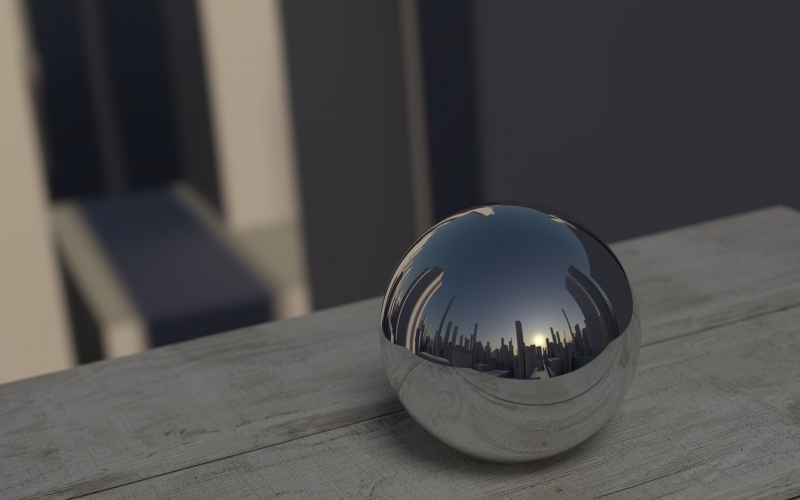
\includegraphics[width=.6\textwidth]{img/pathtracing.png}
				\caption{A photorealistic computer generated image using pathtracing.}%
				\label{fig:pathtracing}%
		\end{floatingfigure}%
		We first send a camera ray through each individual pixel of the image plane and then trace the ray back to a light-source. If a light-source is hit, the pixel gets painted with color, else black. This process is repeated many times over for each pixel and then averaged. A maximum hop number caps the amount of times a ray is able to reflect. A hop number larger than 1 (3 in most simple cases is sufficient, but this is also dependent on the complexity of the scene) allows for some global illumination. Direct consequences of this are soft shadows and ambient occlusion. The reflections and refractions are determined by the BRDF, which essentially determines surface interaction of incoming rays. Through this it is possible to attain caustics and transparency. With each surface a ray hits it carries information from that surface, e.g. its color, and reflects it onto the next surface it hits. This causes color bleeding. Since each pixel is possibly sampled hundreds of thousands of times to reduce the noise that is induced by diffuse reflections, pathtracing may result in a photorealistic render (figure \ref{fig:pathtracing}).
	\subsubsection{Radiosity}
		is a diffuse global illumination method, meaning it is only meant to be used for diffuse surfaces, as it is has been observed to be one of their physical properties. In simple terms, it solves the rendering equation by splitting the objects in cameraspace into patches and treats each of those as a light emitter and receiver. We iteratively check which patches are exposed to light (an initial light-source is required) and adjust their emmitances accordingly until convergence or until we are satisfied with the look of the render (see figure \ref{fig:radiosity}). It takes a while to compute the illumination, but since it is not dependent on the camera view or location, the illumination will stay the same unless an object is moved. Games often preprocess radiosity on scenes with little object movement as it then becomes a quick way of achieving diffuse global illumination \cite{RAD} \cite{RAD3}.
		\begin{figure}[htb!]%
			\begin{center}%
				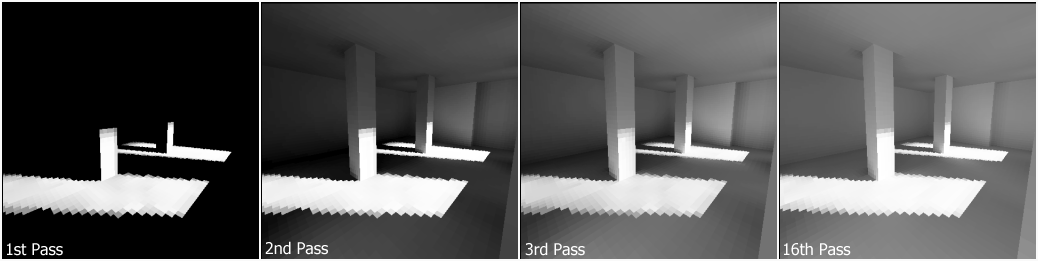
\includegraphics[width=16cm]{img/radiosity.png}
			\end{center}%
			\caption{How radiosity globally illuminates a scene. With each iteration there are more light emitters, meaning that there are more possible patches that can be illuminated. In the first iteration, the only light-emitters are the windows (not visible in the frame). After 16 iterations the scene is sufficiently saturated.}%
			\label{fig:radiosity}%
		\end{figure}%
	\subsection{Computational difficulties of physically based methods}
	With pathtracing we have to take into account thousands of samples of every ray of light with its reflections for all pixels, so the computational difficulty should become apparent \cite{DST}. \\\\
	Radiosity requires a large amount of patches and a moderate amount of iterations to deliver good results. It can be preprocessed and quickly loaded to illuminate a static scene, but would require large amounts of memory to do so. \\\\
	Since physics simulations/animations or games practically always have moving objects or lights per frame, the whole illumination would have to be recomputed for both pathtracing as well as radiosity. Because of this, it is impossible to achieve real time rendering using any of the two methods on an average system. Game engines are forced to stick to achieving global illumination and the visual effects it induces through the application of plausible-looking and efficiently computable techniques. \\\\
	Because of these reasons, it is still conventional to revert to rasterization. Rasterization is a quick method to project 3D objects to a 2D screen, but its speed is achieved by sacrifising realism. \\\\
	A problem that both pathtracing and radiosity do not suffer from is the efficient support of multiple light-sources. This is not always true for rasterization. Fortunately, there are two different rendering methods for rasterization. 

\section{Traditional rendering (rasterization)}
	Graphics pipelines describe each step that has to be taken in order to render an image. It is conventional to use GPU's for applications that rely heavily on rendering images. There is no universal graphics pipeline, because these are dependent on the GPU that is used, which means it is convenient that there exist API's like OpenGL that try to generalize the steps that need to be taken in order to render an image and map them to compatible GPU's. This means that most GPU dependent applications abide by the graphics pipeline as described by, for instance, OpenGL (figure \ref{fig:graphics_pipeline}).
	
	\subsection{Forward rendering}
		With forward rendering, for each object in the scene, we would compute the lighting for its fragments and then render them to the frame-buffer if they pass the z-test (if they are the current frontmost fragment at that x-y-position). As with any 3D scene, it is almost unavoidable that fragments will occlude other fragments. However, we always have to compute the lighting for all fragments, because we do not have full depth information beforehand with forward rendering. The problem here is that if a fragment is not going to be visible anyway, than its lighting computations are effectively useless. This actively prevents the application of multiple light-sources depending on the fragment-count, which in turn depends on the object-count. However, if only few light-sources are applied, this rendering method is preferred, as deferred rendering has some drawbacks when it comes to transparency and anti-aliasing.
		%TODO maybe explain anti aliasing

	\subsection{Deferred rendering}
		\begin{floatingfigure}[r]{.3\textwidth}%
			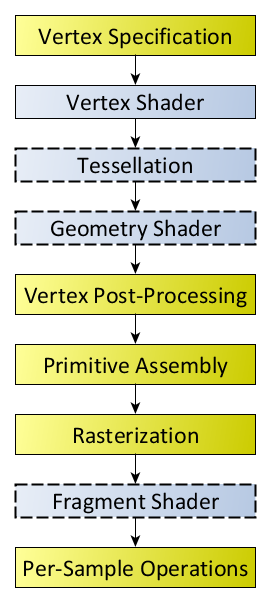
\includegraphics[height=.4\textheight]{img/graphics_pipeline.png}
			\caption{The OpenGL graphics pipeline. The steps within blue boxes are programmable.}%
			\label{fig:graphics_pipeline}%
		\end{floatingfigure}%
		The goal of deferred rendering is to defer lighting calculations until after the frontmost fragments are determined, meaning that geometry and lighting computation are \textbf{decoupled}. This is done by computing necessary geometry buffers (g-buffers) in a first pass through the pipeline that is called "geometry pass" and rendering them into a texture-buffer of the GPU instead of to the screen. In the second pass (lighting pass) all lighting computations are performed using the previously computed geometry that is stored in the texture-buffer. \\\\
		With forward rendering we would have to compute the lighting for every fragment of every object for all light-sources in a single pass. This means that the time complexity of computing forward lighting is $O(amount_{fragments} \cdot amount_{lights})$. \\\\
		If we apply deffered rendering, however, we do not force ourselves to light every fragment as soon as it has been computed. Finding the closest fragment is called "solving the visibility problem". This is done during the geometry-pass when filling the z-buffer with its respective z-values, which can be computed by performing perspective correct interpolation between the vertices of the current polygon (in most cases triangles). The z-buffer, along with all other buffers that are collected, are continuously updated if a closer fragment for the same pixel is found. This will be done in $O(amount_{fragments})$. Now, in the lighting-pass, all the fragments that we light are only going to be lighted once, which would take another $O(amount_{pixels} \cdot amount_{lights})$ of computational time (note that fragments are \textbf{potential} pixels). \\\\
		Decoupling geometry and lighting means decoupling the loops in which geometry and light-sources are iterated. Thus in total, the computational time drops from $O(amount_{fragments} \cdot amount_{lights})$ to $O(amount_{fragments} + amount_{pixels} \cdot amount_{lights})$. This is a huge performance gain if more light-sources are going to be added, at the expense of carrying around g-buffers.
		For all practical purposes, g-buffers have to at least consist of an albedo-buffer, a normal-buffer and a z-buffer. Using at least these g-buffers, it is possible to render an image with basic shading. \\\\

	\subsubsection{Geometry-pass}
		\begin{figure}[]
			\subfigure[]{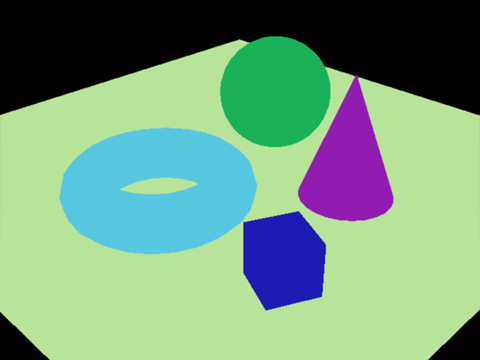
\includegraphics[width=.25\textwidth]{img/wiki_frame_buffer.png}}%
			\subfigure[]{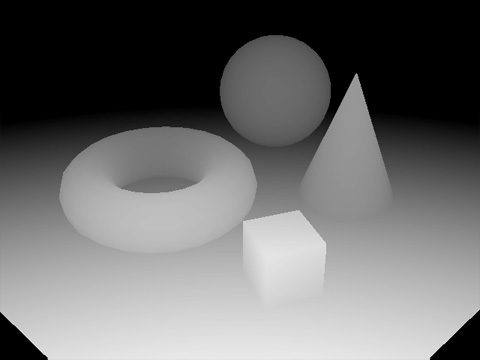
\includegraphics[width=.25\textwidth]{img/wiki_z_buffer.png}}%
			\subfigure[]{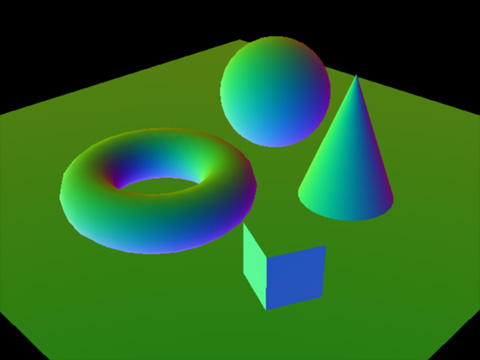
\includegraphics[width=.25\textwidth]{img/wiki_normal_buffer.png}}%
			\subfigure[]{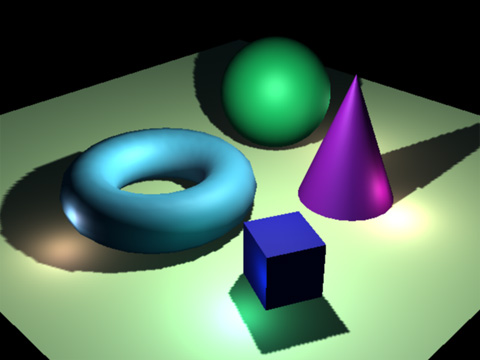
\includegraphics[width=.25\textwidth]{img/wiki_deferred_shading.png}}%
			\caption{An albedo-buffer (a), a z-buffer (b), a normal-buffer (c) and a locally illuminated scene rendered using all of those buffers (d).}
			\label{fig:deferred_shading}%
		\end{figure}

		Each geometry-buffer (g-buffer) stores information of some sort for each individual pixel, meaning that they are all two-dimensional arrays using the dimensions of the screen (screenspace). Note that there are more possible buffers to choose from (position-buffer, stencil-buffer, ...), but these three are the most essential:
		\paragraph{Albedo-buffer}%
			This buffer simply stores the color-values of frontmost fragments. Colors in the context of computer graphics can be referred to as "albedo".% 
		\paragraph{Z-buffer}
			The z-buffer stores depth values of frontmost fragments. These are needed to determine which fragments are closest and visible to the camera. If two different fragments have the same x and y coordinates in screenspace, then the fragment with the smaller z-value in cameraspace is supposed to be in front of the other. This buffer is also used for depth-peeling and screenspace techniques like SSAO\footnote{Screen space ambient occlusion}. 
		\paragraph{Normal-buffer}
			The normal-buffer stores frontmost surface-normals that are mostly used for shading and to determine reflection/refraction directions. They can also be used for light attentuation, since the dot product of a normalized surface-normal and the normalized direction of a light-ray is a criterion for light intensity. If the light-ray is orthogonal to the surface-normal, for instance, the dot product will equal zero, meaning that the light has maximum intensity (lambert reflectance).

	\subsubsection{Lighting-pass} \label{lpass}
		At this point we have to choose a shading technique. Depending on polygon-count we can pick gouraud-shading or phong-shading. \\\\
		Both first compute the normals for each vertex of each polygon in cameraspace. This can be done by averaging the surface normals of the polygons that share the vertex of which the normal is to be computed, which they use for lighting computations. Phong-shading goes one step further and uses its vertex-normals to interpolate the normals of each fragment within the polygons. \\\\
		Gouraud-shading is a fast way of computing shading since it only performs the lighting computations on each vertex of its polygons (which would be three times if the polygons are triangles) as opposed to on each fragment, as well as computing the normal for each fragment, as is done by phong-shading. On the downside, gouraud-shading may look edgy if the 3D models are made of few polygons, which would make phong-shading preferable in that case. \\\\
		Regardless of which shading-technique was chosen, we would have computed all necessary normals in the geometry-pass and stored them in the normal-buffer. In the lighting-pass, we simply read from the normal-buffer and compute the colors for each fragment. This already concludes local illumination, which means we took care of direct lighting.\\\\
		By now it should become apparent why lighting in a single pass with multiple light-sources is inefficient, since all of the illumination computations would be in vain if the visibility test does not pass anyway. The g-buffers that we collect in the geometry pass make this possible. 

\section{Visual effects} 
	\begin{floatingfigure}[l]{.5\textwidth} %
		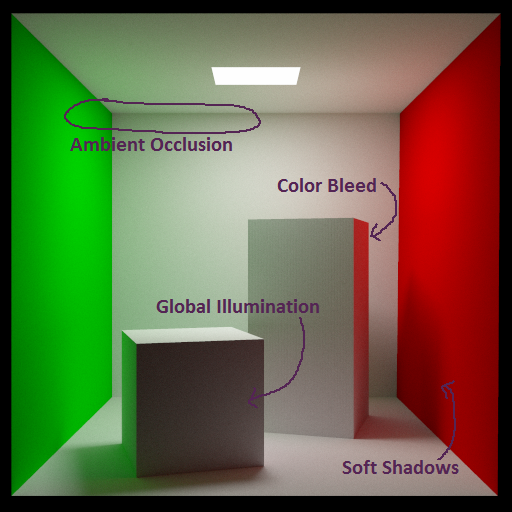
\includegraphics[width=.5\textwidth]{img/visual_effects.png} %
			
		\caption{Diverse visual effects caused by global illumination inside a cornell box. The image was rendered using pathtracing.}%
		\label{fig:visual_effects}%
	\end{floatingfigure} %

	The following are visual effects that are sought after, since they are fundamental to conveying realism. If the scene was globally illuminated, all of these visual effects would be visible in some way or another, so naturally the problem lies within simulating all of those visual effects efficiently. \\\\
	Unfortunately, since with traditional rendering we mostly only use the aforementioned shading-methods (\ref{lpass}), we are forced to apply further techniques to attain all of those visual effects in order to approximate a globally illuminated scene. \\\\
	With pathtracing and radiosity, the simulation of all of those visual effects is built-in within their rendering techniques, though at the expense of reaching non-interactive framerates. \\\\
	Next to the basic visual effects in figure \ref{fig:visual_effects}, there is depth-of-field and motion-blur. Those will not be covered in this paper, as they are visual effects induced by the camera as opposed to lighting. Nevertheless, they can also be simulated.

	\subsection{Ambient occlusion}
		\begin{floatingfigure}[r]{.5\textwidth}%
			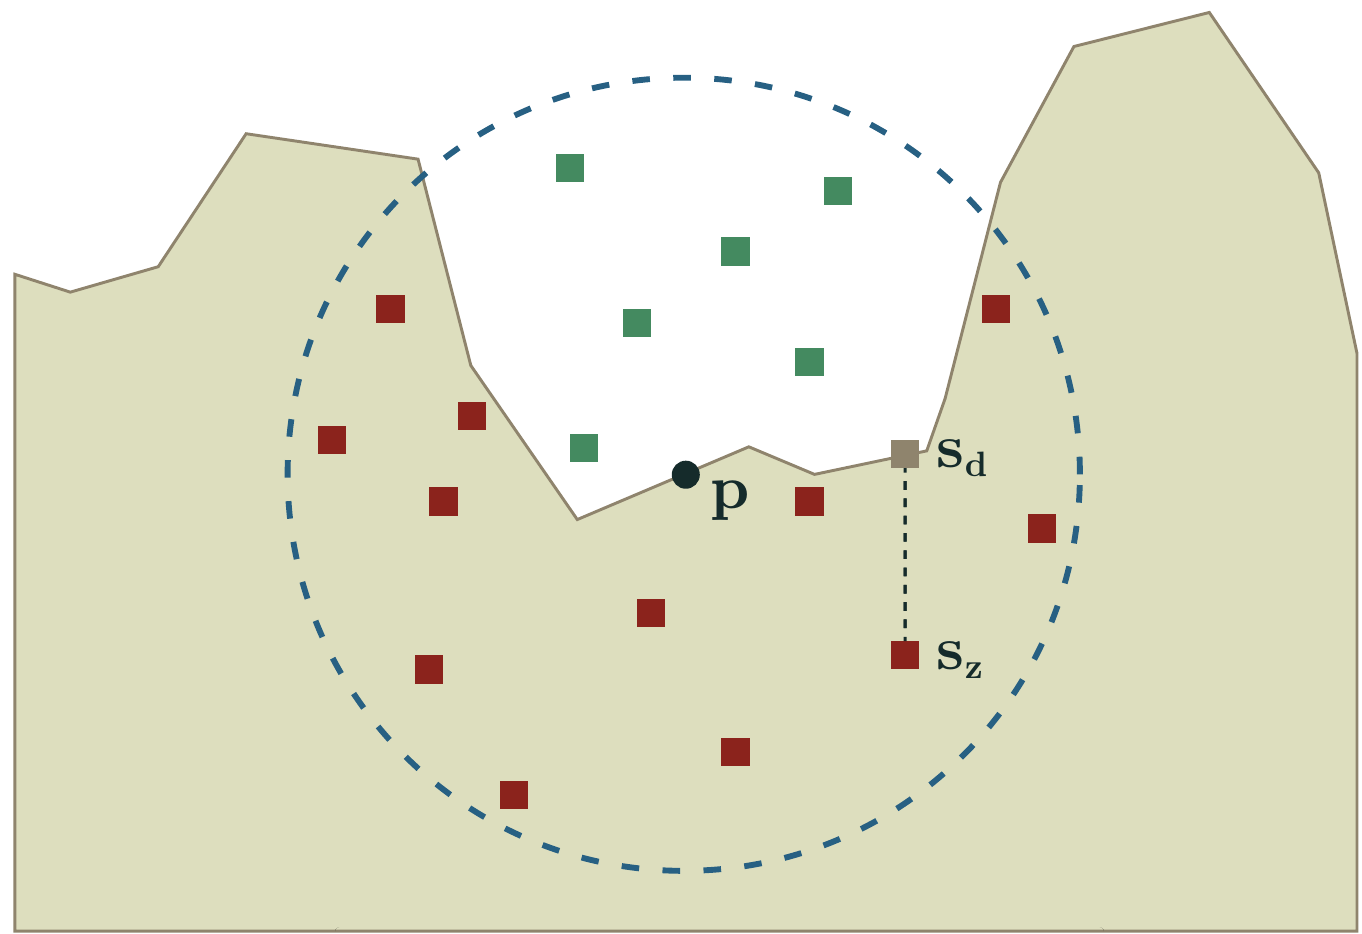
\includegraphics[width=.5\textwidth]{img/ao_sphere_sampling.png}%

			\caption{Computing the ambient occlusion factor $AO$ via sphere sampling.}%
			\label{fig:ao_sphere_sampling}%
		\end{floatingfigure}%


		%TODO explain sphere sampling, hemispheresampling insert images of those
		Ambient occlusion (the visual effect) essentially describes how likely it is that a surface is occluded, meaning that light cannot reach it because some other surface is in the way (figure \ref{fig:visual_effects}) \cite{AOM}. This effect can be efficiently approximated by using a method called \textbf{screen space ambient occlusion (SSAO)}. \\\\
		
		This method basically samples points in a sphere around each z-value $p$ of the z-buffer $Z$. Given a z-value $p$, a radius $r$ and a sampling count $N$ we can compute the ambient occlusion factor $AO$ by checking $N$ randomly picked surrounding points $S$ within $r$:
		\\\\
		$$ AO = \frac{1}{N} \Sigma_{i}^{N} O(p, S_i) $$

		where $O(b)$ returns $1$ if point $b$ is occluded, else $0$:

		\[
			O(b) = 
			\begin{dcases*} 
			\text{1,} & if  $b_{z} \leq Z_{b_{x}, b_{y}}$ \\ 
			\text{0,} & otherwise 
			\end{dcases*} 
		\]

		Since with deferred rendering we also have a normal-buffer, we can use those normals to do hemi-sphere sampling instead, because with sphere-sampling, on average, half of the samples would be occluded. By applying hemi-sphere sampling we can cut the sample-count in half, which will result in a performance increase. \\\\
		The final $AO$ factors can be put in a texture-buffer to be used in post-processing or they can be used directly. To apply ambient occlusion to the final image, the $AO$ values are multiplied with their respective pixels in the frame-buffer. Because $0 \leq AO \leq 1$ this can be seen as tweaking the intensity of the color on a specific pixel. \\\\
		Since it only runs over the z-buffer it is considered screen space. Ambient occlusion (the visual effect) is an effect directly caused by global illumination, leading the ambient occlusion (method) to be considered a necessity for simulating global illumination. \\\\

	\subsection{Color bleeding}
		Color bleeding happens when light directs information from one hit-surface to another. Let A and B be objects. If A reflects light onto B and A's surface is blue, then B will also appear
		to be slightly blue on the reflected area. To have this happen it would obviously be convenient to trace rays of some sort. Point-based color bleeding approximates this by using point cloud surfels with direct illumination values \cite{PBCB}.

	\subsection{Soft shadows}
		We can easily compute hard shadows in screen space using shadow mapping. A shadow map is a buffer that contains the distances between the light source and all pixels (visible fragments) of the scene. Having created the shadow map we check if the entry in the z-buffer is larger than the entry in the shadow map. If so, then the fragment is in shadow and is painted black. If not, then the fragment keeps its color and we can proceed to compute its local illumination. This can be extended to soft shadows simply by blending together fragments in shadow with their surrounding fragments.

	\subsection{Reflection} \label{sec:reflection}
		\begin{floatingfigure}[r]{.7\textwidth}%
			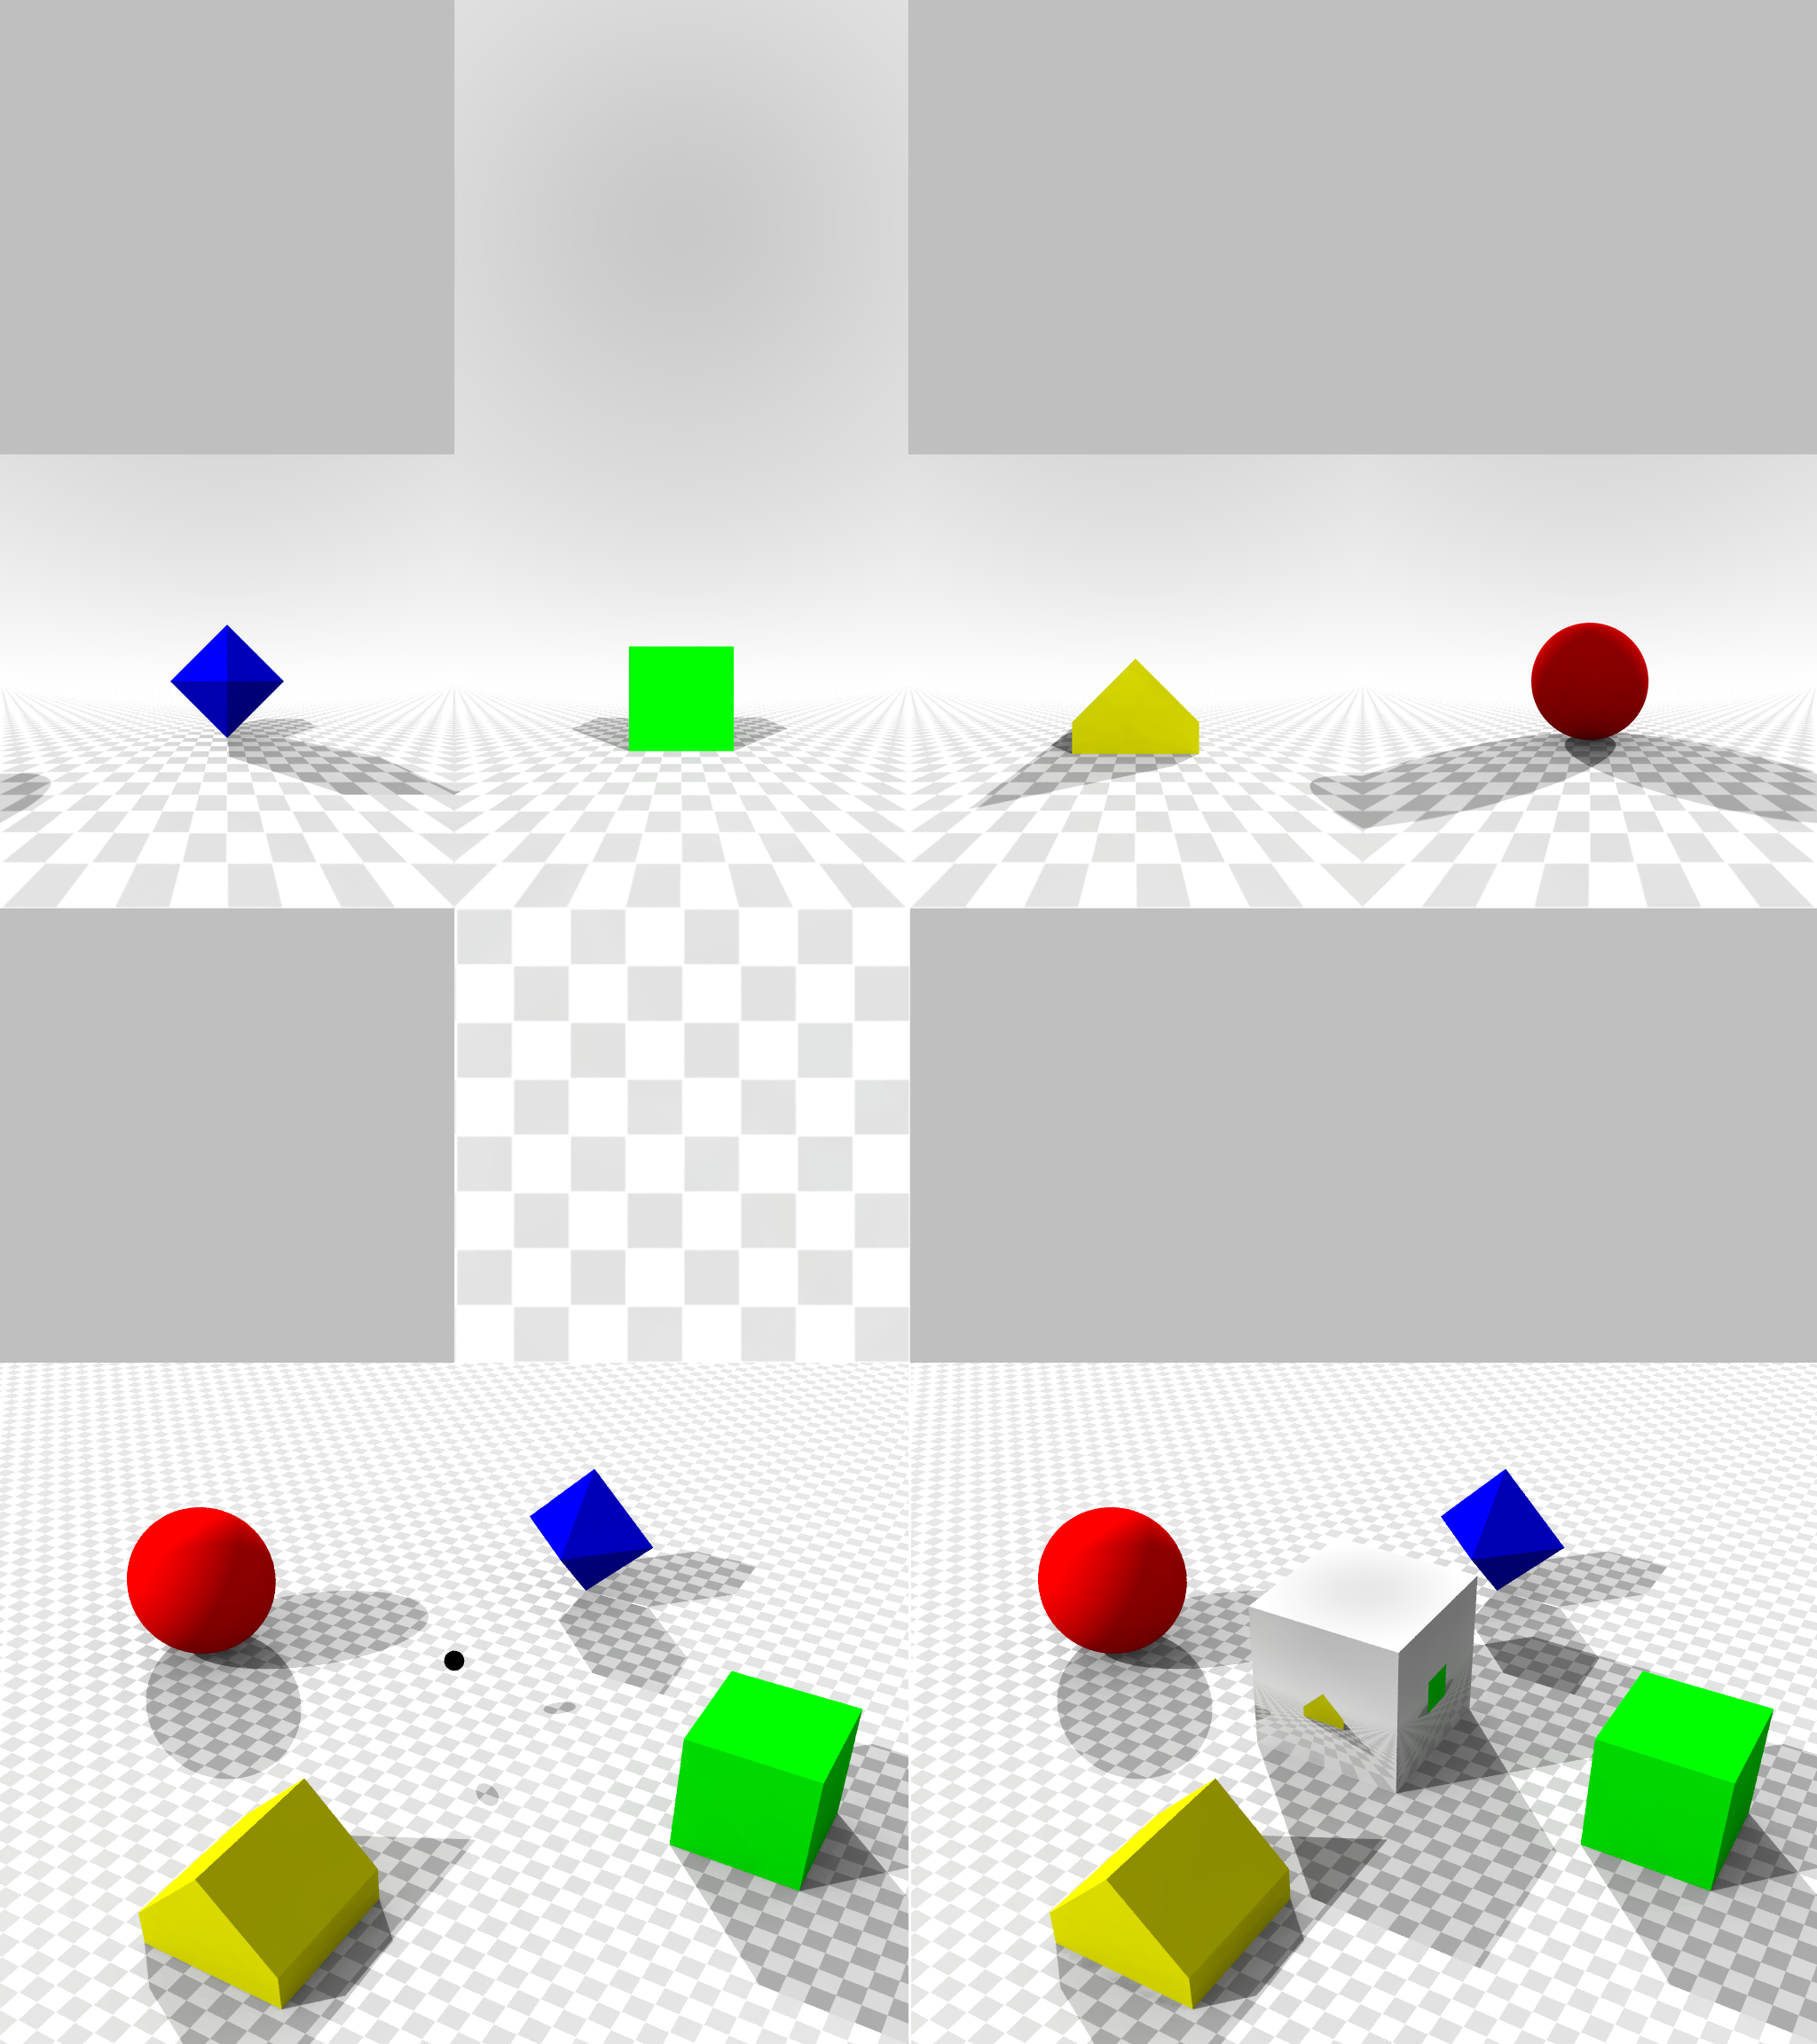
\includegraphics[width=.7\textwidth]{img/cube_map.png}
			\caption{How a cube-map is rendered. The black sphere in the lower image represents the camera. The resulting six renders are put together in the cube-map in the upper image.}%
			\label{fig:cube_map}%
		\end{floatingfigure}%
		Reflections can be efficiently computed. If the reflective surface is completely planar, then we can simply project the texture that is supposed to be reflected onto the surface that reflects it. In all other cases, we rely on \textbf{cube-mapping}. \\\\
		Creating a cube-map (figure \ref{fig:cube_map}) works like this: we define a cube with our camera in its center. Next, we treat each plane of the cube as an image plane that we render to, meaning we render six times in total, and save those inside a buffer. This buffer now has knowledge about the entire surrounding environment of the reflective object. When computing the color of a vertex of a reflective object, we use the direction vector from the camera to the vertex and use the vertex-normal to get the specular reflection direction, which will ultimately point at the spot on the cube-map that will be reflected. The issue with this is that it lacks the ability to self-reflect \cite{REFL}. \\\\

\section{Deep g-buffer}
	Deep g-buffers make use of a concept similar to depth peeling. Instead of storing information about the closest surface, in an n-layer deep g-buffer we also store information about the n-closest surface \cite{Mara2016DeepGBuffer}. \\\\
	Practical observations suggest that the second-closest surface is often not the second-most relevant for shading and visual effects \cite{Mara2016DeepGBuffer}. To resolve this issue we rely on minimum depth separation, which essentially introduces a distance $\Delta z$ that has to be exceeded when looking for the next-closest surface immediately after the current one. Setting $\Delta z = 0$ makes the generated 2-layer z-buffer of the deep g-buffer turn into a 2-layer k-buffer\footnote{K-layer z-buffer that stores the z-values of the k-closest polygons in order} \cite{MFEKB}. \\\\
	How to pick $\Delta z$ ultimately depends on the depth complexity of the scene and has to be tweaked accordingly. If $\Delta z$ is too large, it is possible that important visual information might be missed. On the other hand, if $\Delta z$ is too small, it is possible that unnecessary information might be picked up. According to NVIDIA, $\Delta z = 50cm$ seems to consistently deliver stable results, at least in the renders done in their paper \cite{Mara2016DeepGBuffer}.
	\subsection{Generating a 2-layer deep g-buffer}
		NVIDIA proposes two ways of generating a 2-layer deep g-buffer, one of which is straight forward to help demonstrate the idea and one of which is efficient. \\\\
		The first one is called "Strawman Two-Pass Generation Algorithm" and displayed in algorithm \ref{alg:two_pass_strawman}. $Z$ is the 2-layer z-buffer, $S(x, y, z)$ returns other g-buffers needed for shading and $T(tri)$ applies the transformation $T$ to triangle $tri$ (model-view-projection and skinning-transformations). In the first pass we simply collect the first layers g-buffers and in the second pass we peel away the first layers g-buffers to receive the second layer. Since fragments get discarded if their distance to the previous fragment is smaller than $\Delta z$ the minimum depth seperation constraint is met. \\\\
		This is essentially two-pass depth peeling, however, there is a more efficient algorithm which only requires a single pass displayed in \ref{alg:one_pass_strawman}. \\\\
		In order to save a pass over the geometry, we rely on an oracle that predicts the first layers z-buffer before it is even rendered. Using that prediction, we can compute fragments for the second layer by peeling the first layer. In total, there are four variants to go about this. $t$ is the index of the frame.
		%TODO go more into detail how frames from the animation as recycled as approximation
		\begin{enumerate}
			\item \textbf{DELAY VARIANT} manages to predict the first layers z-buffer by adding a frame of latency, meaning that what is happening in the scene (animations, object movements and such) and what is being rendered on the screen is out of sync by one frame. This way, the next frames transformation $T_{t+1}$ is known at render time, enabling us to predict first layer z-buffers perfectly (since we do not really predict it anyway). The downside to this is, obviously, the frame latency.

			\item \textbf{PREVIOUS VARIANT} approximates the first layer z-buffer by taking the previous frames first layer z-buffer. This will deliver good results if camera- and object-movement are minimal, but even then, the errors would appear in the second layer, which is not visible to begin with (excluding transparent objects). It does not guarantee minimum separation.

			\item \textbf{PREDICT VARIANT} uses velocities from the underlying physics simulation or animation to predict the next transformation $T_{t+1}$. Alternatively, extrapolation over the change in vertices from the previous and current frame would also work. Accurate velocity prediction will deliver accurate results without latency. In the other case, drawbacks are equivalent to that of the \textit{PREVIOUS VARIANT}

			\item \textbf{REPROJECT VARIANT} performs the minimum separation test against the first layer z-buffer of the previous frame. The visibility test is done using screen coordinates and z-values computed using the vertices of the previous frame, meaning the visibility test is done in the "past". Like with \textit{PREDICT VARIANT}, moving objects are a source of error, but the velocities computed in this case are perfect, which means the errors are not as bad. Benchmarks suggest that compared to all the other variants, this delivers the most stable performance at the greatest speed.

		\end{enumerate} 
		%TODO pretty the alogirhtms
		\begin{algorithm} \label{alg:two_pass_strawman} \caption{Strawman two-pass generation algorithm for generating 2-layer deep g-buffers}
		\begin{lstlisting}[frame=single]
//1st pass
submit geometry with:
  geometryShader(tri):
    emit T(tri) to layer 0
  pixelShader(x, y, z):
    return S(x, y, z)

//2nd pass
submit geometry with:
geometryShader(tri):
    emit T(tri) to layer 1
  pixelShader(x, y, z):
    if z > Z[0][x][y] + \Delta z:
      return S(x, y, z)
    else:
      discard fragment
		\end{lstlisting}
		\end{algorithm}
		 
		\begin{algorithm} \label{alg:one_pass_strawman} \caption{An improved one-pass algorithm for generating 2-layer deep g-buffers}
		%TODO pretty the alogirhtms
		\begin{lstlisting}[frame=single]
submit geometry with:
  geometryShader(tri)
    emit T(t, tri) to layer 0
    emit T(t, tri) to layer 1
  if (VARIANT == Delay) or (VARIANT == Predict):
    emit T(t+1, tri) to layer 2
  pixelShader(x, y, z):
    switch (layer):
      case 0: // 1st layer; usual G-buffer pass
        return S(x, y, z)
      case 1: // 2nd G-buffer layer: choose the comparison texel
        if (VARIANT == Delay) or (VARIANT == Predict):
          L = 2 // Comparison layer
          C = (x, y, z) // Comparison texel
        else if VARIANT == Previous:
          L = 0; C = (x, y, z)
        else if VARIANT == Reproject:
          L = 0; C = (x[t-1] , y[t-1], z[t-1])
        if z C > Z[t-1] [L][x[C], y[C] ] + delta_z: return S(x, y, z)
        else: discard the fragment
      case 2: // Depth only write to predict Z[t+1][0]; no shading
        return // We only reach this case for Delay and Predict
		\end{lstlisting}
		\end{algorithm}
	\subsection{Global illumination using 2-layer deep g-buffer} 
		%maybe explain ambient light
		To simulate global illumination we combine direct-light $DIRECT$, ambient-light $AMBIENT$, screen space ambient visibility\footnote{$AV = 1-AO$} $AV$ as well as screen space radiosity $RADIOSITY$ and screen space reflections $REFLECTIONS$ by \cite{RSM} \cite{TSTMT}
		$$ DIRECT + AV \cdot AMBIENT + RADIOSITY + REFLECTIONS $$
		
	\subsection{Double screen space ambient occlusion using 2-layer deep g-buffer}
		Scalable ambient obscurance \cite{SAO}, which is an ambient occlusion method, is extended to work with deep g-buffers. To take into account both z-buffers of the deep g-buffer we have
		$$ AO(X) = \sqrt{\frac{\pi}{N} \Sigma_{i=1}^{N} max(0, A_{i}^{0}, A_{i}^{1})} $$
		for the ambient occlusion factor $AO$ where $N$ is the sample count, $R(Z, i)$ returns the position of the $i'th$ sample surface using the z-buffer $Z$ and
		$$ A_{i}^{j} = O(X, R(Z[j], i))$$
		where $X$ is the position of the z-value that is being checked, $Y$ the position of the sample (a surrounding z-value) and
		$$ O(X, Y) = (1 - \frac{v \cdot v}{r^2}) \cdot max(\frac{v \cdot n_X - \beta}{\sqrt{v \cdot v + \epsilon}}, 0) $$
		evaluates if the z-value at $Y$ is occluded by z-value at $X$, where $r$ is the sample radius, $v = Y - X$ the direction vector from position $X$ to position $Y$ and $n_X$ is the normal-vector in the normal-buffer at position $X$. \\\\
		With the 2-layer deep g-buffers accounted for, SAO now produces a less noisy $AO$ factor with more plausible shading-falloff \cite{Mara2016DeepGBuffer}. 
		%TODO explain benefits with images (like in presentation). explain halos with normal ssao and how they are fided with double ssao
		
	\subsection{Double screen space radiosity using 2-layer deep g-buffer}
		We extend screen space radiosity \cite{RTAII} to 2-layer deep g-buffers. We have 
		$$ E(X) = \int_{\Omega} \frac{B(Y)}{\pi} max(n_X \cdot \omega, 0) d\omega$$
		for the incident irradiance at $X$ caused by the outgoing diffuse radiance $B(Y)$ from the closest point $Y$ in direction $\omega = Y - X$. This can be \textbf{numerically estimated} by
		$$ E(X) = \frac{2\pi}{M} \Sigma_{samples} B(Y) max(\omega \cdot n_X, 0)$$
		where $\omega$ is normalized. \\\\
		We sample $N$ points $Y$ from both g-buffer layers while only using the $M$ points for which
		$$ (\omega \cdot n_X) > 0 $$
		and
		$$ (\omega \cdot n_Y) < 0 $$. Skipping this test will cause bias (noise), but at the same time makes it possible to take more samples, which in return reduces variance. This is up to the users preference. \\\\
		$$ B(X) = E(X) \cdot p_X \cdot boost(p_x) $$
		is the reflected outgoing radiance caused by the incident irradiance at $X$, where $p_X$ is the diffuse reflectivity at $X$, which is amplified by 
		$$ boost(p) = \frac{max_{\lambda}p[\lambda] - min_{\lambda}p[\lambda]}{max_{\lambda}p[\lambda]} $$ 
		where $\lambda$ is the wavelength or color channel. Choosing $boost(p) = 1$, for instance, will conserve energy. Else it can be used to boost the scattering of radiance of a saturated surface, which will cause a stronger color bleed. \\\\
		Since not all points in the deep g-buffer produce robust approximations for indirect shading, we compute a confidence value $0 \leq M/N \leq 1$ that indicates how many samples contribute to the final result, with a larger confidence value implying stronger influence. According to the confidence value, we linearly interpolate between a precomuted lighting solution and indirect deep g-buffer illumination. \\\\
		Iteratively repeating the above steps across frames will result in multi bounce indirect illumination, causing soft shadows and color bleeding and diffuse global illumination. This is done by computing one bounce per frame, using the previous frames irradiance-buffer $E_{t-1}$, which would simulate $n$ bounces in $n$ frames. Obviously this method is prone to ghosting, but its effect can be reduced by damping the forwarded irradiance-buffer by a factor $0 < \delta \leq 1$, which in simple words "underestiamtes" illumination. Compensation for this is provided by some environmental lighting from static light probes. The same accumulation procedure is done across deep g-buffer layers. \\\\
		Finally, to account for any remaining noise due to undersampling, \textbf{temporal filtering} is applied by
		$$ E_t = E(1 - \alpha) + reproject(E_{t-1}) \alpha $$
		if for the pixel the reprojected point is within $1cm$ of either layer, else
		$$ E_t = E $$
		with the purpose of detecting faulty velocity approximations and discarding accordingly. Nvidia recommends $\alpha = 0.85$ in most occasions, as $\alpha \geq 0.95$ causes lighting latency and artifacts.
		%TODO explain benefits with images (like in presentation) insert statue color bleeding image

	\subsection{Mirror reflections using 2-layer deep g-buffer}
		Screen space reflections are adapted to deep g-buffers by reflection raytracing. Each point in cameraspace is projected into the two g-buffer layers via reflection rays, where points with a maximum distance of $\Delta z$ within both layers are treated as a hit. The outgoing radiance is set equal to the incoming radiance along the reflection direction. If this procedure fails, e.g. if after a maximum distance of $d > \Delta z$ there is still no hit, or if the reflection ray reaches void space, one performs a switch to environmental mapping as described in section \ref{sec:reflection}.
		%TODO explain benefits with images (like in presentation). insert flying duckreflection image

\section{Conclusion}
	Deep g-buffers do a good job at approximating global illumination in real time. The resulting renders cover more details than renders which use only a single layer of information. As stated by NVIDIA, deep g-buffers also have potential to be used for transparency, depth of field and motion blur.%TODO cite

	\begin{figure}[htb!]%
		\begin{center}%
			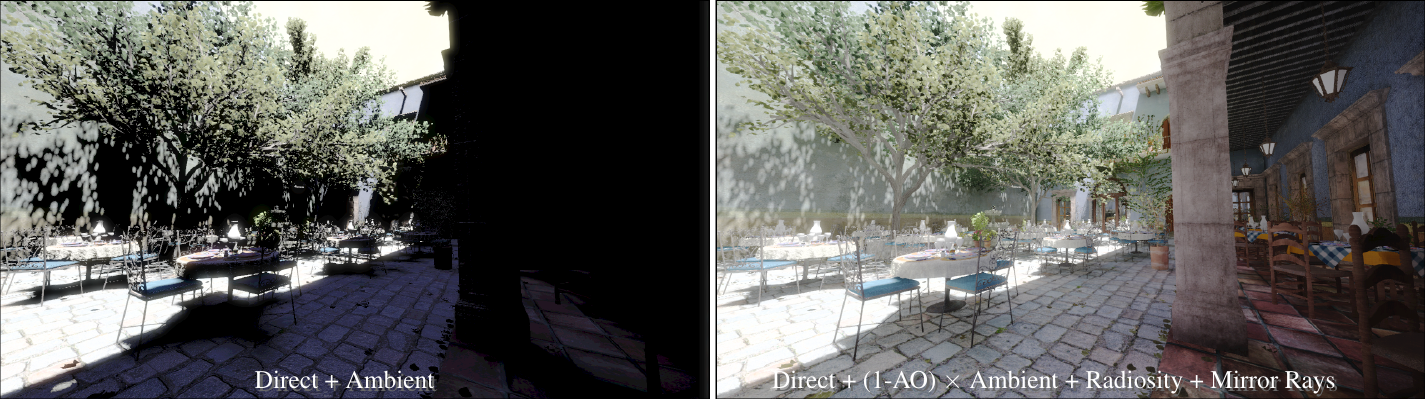
\includegraphics[width=16cm]{img/deep_g_buffer_render.png}
		\end{center}%
		\caption{An image rendered without (left) and with the usage of 2-layer deep g-buffers (right). The image was generated in 10.8ms at 1080p using NVIDIA GeForce 980, which implies a theoretical framerate of 92 frames per second.}%
		\label{fig:deep_g_buffer_render}%
	\end{figure}%

%%%%%%%%%%%%%%%%%%%%%%%%%%%%%%%%%%%%%%%%%%%%%%%%%%%%%%%%%%%%
% Bibliography
\printbibliography

\end{document}